\subsection{Possible data augmentation techniques}

\subsubsection{Core concepts}
\paragraph{CNN - Convolutional Neural Network}\mbox{}\\

Convolutional neural networks are used to extract intermediate representations of the input. They take advantage of convolutional filters with weights that are learned during training. Such convolutional filters create a convolutional layer. An image passed through a first convolutional layer creates the feature maps. Convolutional layers can be stacked together, creating in the result a convolutional network.
Convolutional layers are usually combined with subsampling techniques, such as pooling. 

\begin{figure}[H]
    \centering
    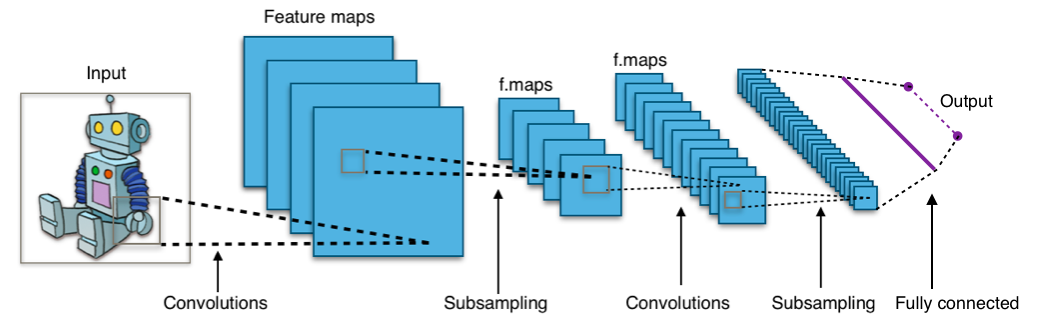
\includegraphics[width=\linewidth]{concept_engineering/Typical_cnn.png}
    \caption{Typical architecture of a convolutional neural network\cite{cnn-typical}.}
    \label{fig:cnn}
\end{figure}


\paragraph{Autoencoder}\mbox{}\\
\begin{figure}[H]
    \centering
    \begin{tikzpicture}[
    box/.style={draw, minimum width=2cm, minimum height=3cm, text width=1.8cm, align=center},
    smallbox/.style={draw, minimum width=1.5cm, minimum height=1.2cm, text width=1.3cm, align=center},
    arrow/.style={->, >=latex, thick},
    label/.style={font=\small}
]

% Components
\node[circle, draw] (input) {Input $x$};
\node[box, right=1cm of input] (encoder) {Encoder};

% Latent space
\node[right=1cm of encoder] (latent) {};
\node[circle, draw, minimum size=1cm, right=0cm of latent] (z) {$z$};

\node[box, right=1cm of z] (decoder) {Decoder};
\node[circle, draw, right=1cm of decoder] (output) {Output $\hat{x}$};

% Reparameterization trick

% Connections
\draw[arrow] (input) -- (encoder);
\draw[arrow] (encoder) -- (z);
\draw[arrow] (z) -- (decoder);
\draw[arrow] (decoder) -- (output);

% Labels
\node[label, below=0.2cm of input] {High-dimensional};
% \node[label, above=0.2cm of mu] {Latent space};
\node[label, below=0.2cm of output] {Reconstructed};

% KL Divergence

% Reconstruction Loss
\draw[<->, >=latex, bend right=30] ($(input.south west)+(1,-0.3)$) to node[below, font=\small] {Reconstruction Loss} ($(output.south east)+(-1.3,-0.2)$);
\end{tikzpicture}
    \caption{Visualization of an autoencoder. Circles are tensors, rectangles neural networks.}
    \label{fig:autoencoder}
\end{figure}
\indent Autoencoder is an architecture of deep learning model that consists of two deep neural networks - Encoder and Decoder. The task of the encoder is to transform the input into latent representation of the input. Usually it compresses it, for example to a vector or smaller matrix/tensor. Decoder then takes such latent representation and transforms it back to its original form. 

The loss function between input $x$ and output $\hat{x}$ is usually one of the following: L1, L2, MSE.

\paragraph{U-Net}\mbox{}\\
\indent U-Net is a special type of convolutional neural network, originally built for the task of image segmentation, especially in medical imaging. Its architecture resembles a U-shape, similar to an autoencoder. The encoder on the left side reduces the input image size while capturing significant features. The right side increases resolution and performs tasks like segmentation, utilizing the features extracted by the encoder via "skip connections." Despite the similarity, U-Net is not considered an autoencoder due to the use of skip connections.

\begin{figure}[H]
    \centering
    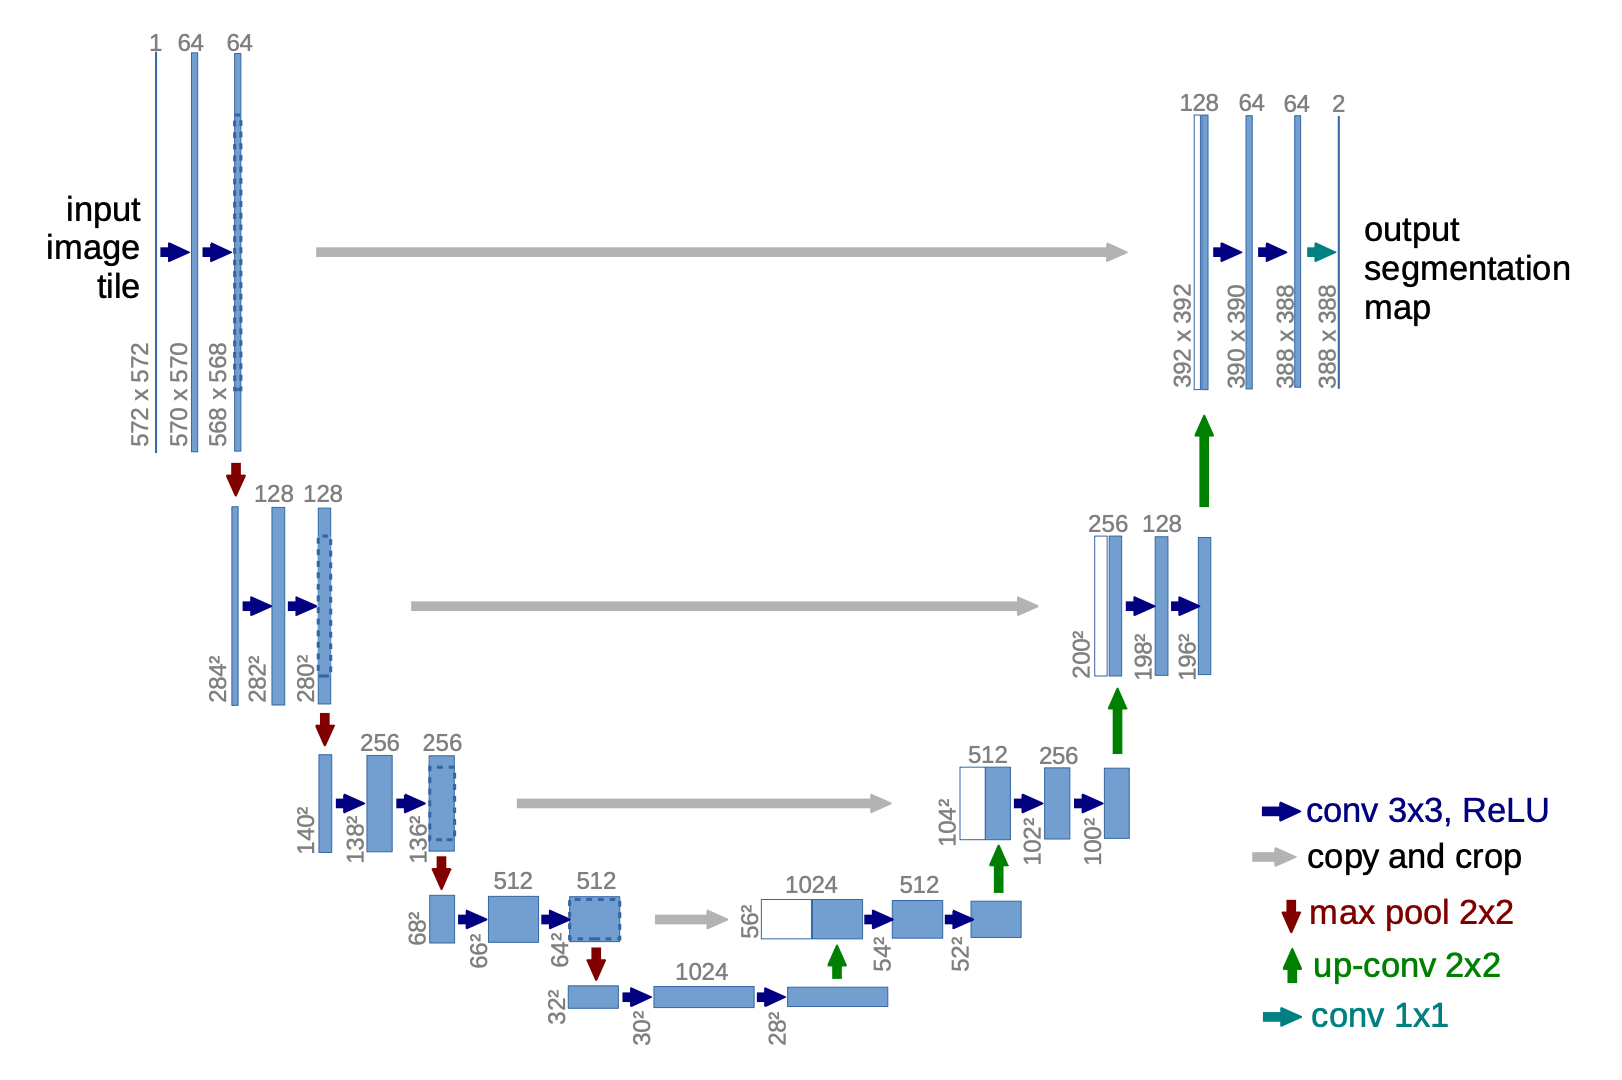
\includegraphics[width=0.9\linewidth]{concept_engineering/unet/U-net.png}
    \caption{U-Net architecture\cite{RFB15a}.}
    \label{fig:unet}
\end{figure}



\newpage
\subsubsection{GANS}

\begin{figure}[H]
    \centering
    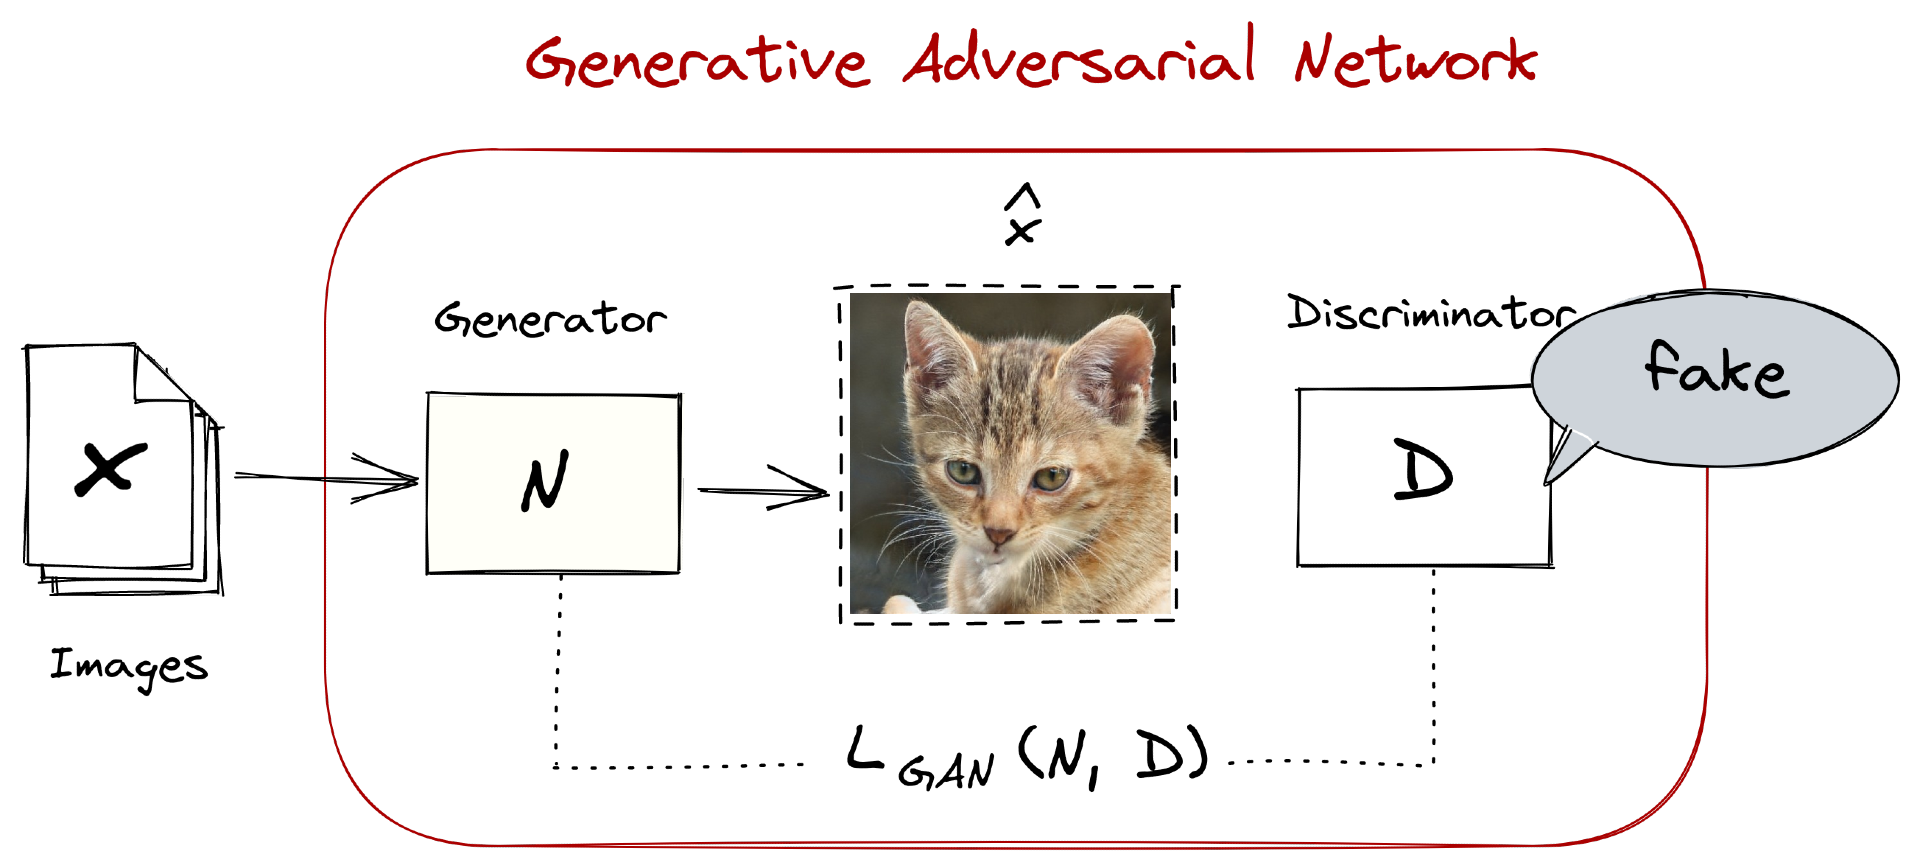
\includegraphics[width=0.9\linewidth]{concept_engineering/vqgan/vqgan_gan_inside.png}
    \caption{Caption}
    \label{fig:gan}
\end{figure}

Generative Adversarial Networks (GANs) are deep learning models that consist of two neural networks.
The first is a generator \( G \), which is responsible for generating false samples from random noise, and the second is a discriminator \( D \), which tries to detect which samples are false.
The generator and the discriminator compete in a minimax game. The two networks are trained simultaneously with opposite goals.

Mathematically, the goal of GANs is represented by the following minimax objective function:

\begin{equation}
\min_G \max_D V(D, G) = \mathbb{E}_{x \sim p_{data}(x)}[\log D(x)] + \mathbb{E}_{z \sim p_z(z)}[\log (1 - D(G(z)))]
\end{equation}
where:

\begin{itemize}
\item \( D(x) \) represents the probability that the discriminator correctly identifies a real sample \( x \),

\item \( G(z)=\hat{x} \) represents the synthetic data generated by the generator from random noise \( z \), in our case CT scan,

\item \( p_{data}(x) \) is the data distribution of the real samples,

\item \( p_z(z) \) is the distribution of the random noise input to the generator.
\end{itemize}

\paragraph{Loss function}\mbox{}\\
\indent GAN loss function can be calculated as
\begin{equation}
    L_{GAN}(N,D) = [\log D(x) + log(1-D(\hat{x}))]
\label{loss_gan}
\end{equation}
However it often leads to discriminator being too good on the beginning and in result generator stops training. To mitigate that, each neural network, generator and discriminator has their own loss.
The loss function of the discriminator is typically defined as

\begin{equation}
L_D = - \left( \mathbb{E}_{x \sim p_{data}(x)}[\log D(x)] + \mathbb{E}_{z \sim p_z(z)}[\log (1 - D(\hat{x}))] \right)
\end{equation}


This loss encourages the discriminator to maximize its ability to distinguish real from false data. On the other hand, the generator loss function can be defined as


\begin{equation}
L_G = - \mathbb{E}_{z \sim p_z(z)}[\log D(\hat{x})]
\end{equation}


This loss encourages the generator to improve the quality of the false samples by "fooling" the discriminator into classifying them as real. Training continues until the generator produces samples that are indistinguishable from the real data, at which point the discriminator cannot distinguish between real and generated samples and a Nash equilibrium\footnote{\url{https://en.wikipedia.org/wiki/Nash_equilibrium}} is reached.

GANs have had a significant impact in areas such as image generation, data augmentation and even super-resolution tasks, but their training can be unstable due to problems such as vanishing gradients. 


\paragraph{Generation of CT scan}\mbox{}\\

To generate an artifical CT scan using GAN, one should sample a Gaussian noise tensor $z$ from $\mathcal{N}(0,1)$, of shape the same as the generator input, and then pass it to a generator, which would produce a synthetic CT scan as a result.
\newpage
\subsubsection{Diffusion}
% \paragraph{Forward diffusion process}\mbox{} \\
% \begin{equation}
%     q(\mathbf{x}_{t}|\mathbf{x}_0)=\mathcal{N}(\mathbf{x}_{t};\sqrt{\bar{\alpha}_{t}}\mathbf{x}_0,(1-\bar{\alpha}_{t})\mathbf{I})
% \end{equation}

% \begin{equation}
% \mathbf{x}_{t}=\sqrt{\alpha_{t}}\mathbf{x}_{t-1}+\sqrt{1-\alpha_{t}}\boldsymbol{\epsilon},\quad\boldsymbol{\epsilon}\sim\mathcal{N}(0,\mathbf{I}).
% \end{equation}

% \begin{aligned}
% \mathbf{x}_t 
% &= \sqrt{\alpha_t}\mathbf{x}_{t-1} + \sqrt{1 - \alpha_t}\boldsymbol{\epsilon}_{t-1} & \text{ ;where } \boldsymbol{\epsilon}_{t-1}, \boldsymbol{\epsilon}_{t-2}, \dots \sim \mathcal{N}(\mathbf{0}, \mathbf{I}) \\
% &= \sqrt{\alpha_t \alpha_{t-1}} \mathbf{x}_{t-2} + \sqrt{1 - \alpha_t \alpha_{t-1}} \bar{\boldsymbol{\epsilon}}_{t-2} & \text{ ;where } \bar{\boldsymbol{\epsilon}}_{t-2} \text{ merges two Gaussians (*).} \\
% &= \dots \\
% &= \sqrt{\bar{\alpha}_t}\mathbf{x}_0 + \sqrt{1 - \bar{\alpha}_t}\boldsymbol{\epsilon} \\
% q(\mathbf{x}_t \vert \mathbf{x}_0) &= \mathcal{N}(\mathbf{x}_t; \sqrt{\bar{\alpha}_t} \mathbf{x}_0, (1 - \bar{\alpha}_t)\mathbf{I})
% \end{aligned}

\begin{figure}[h]
    \centering
    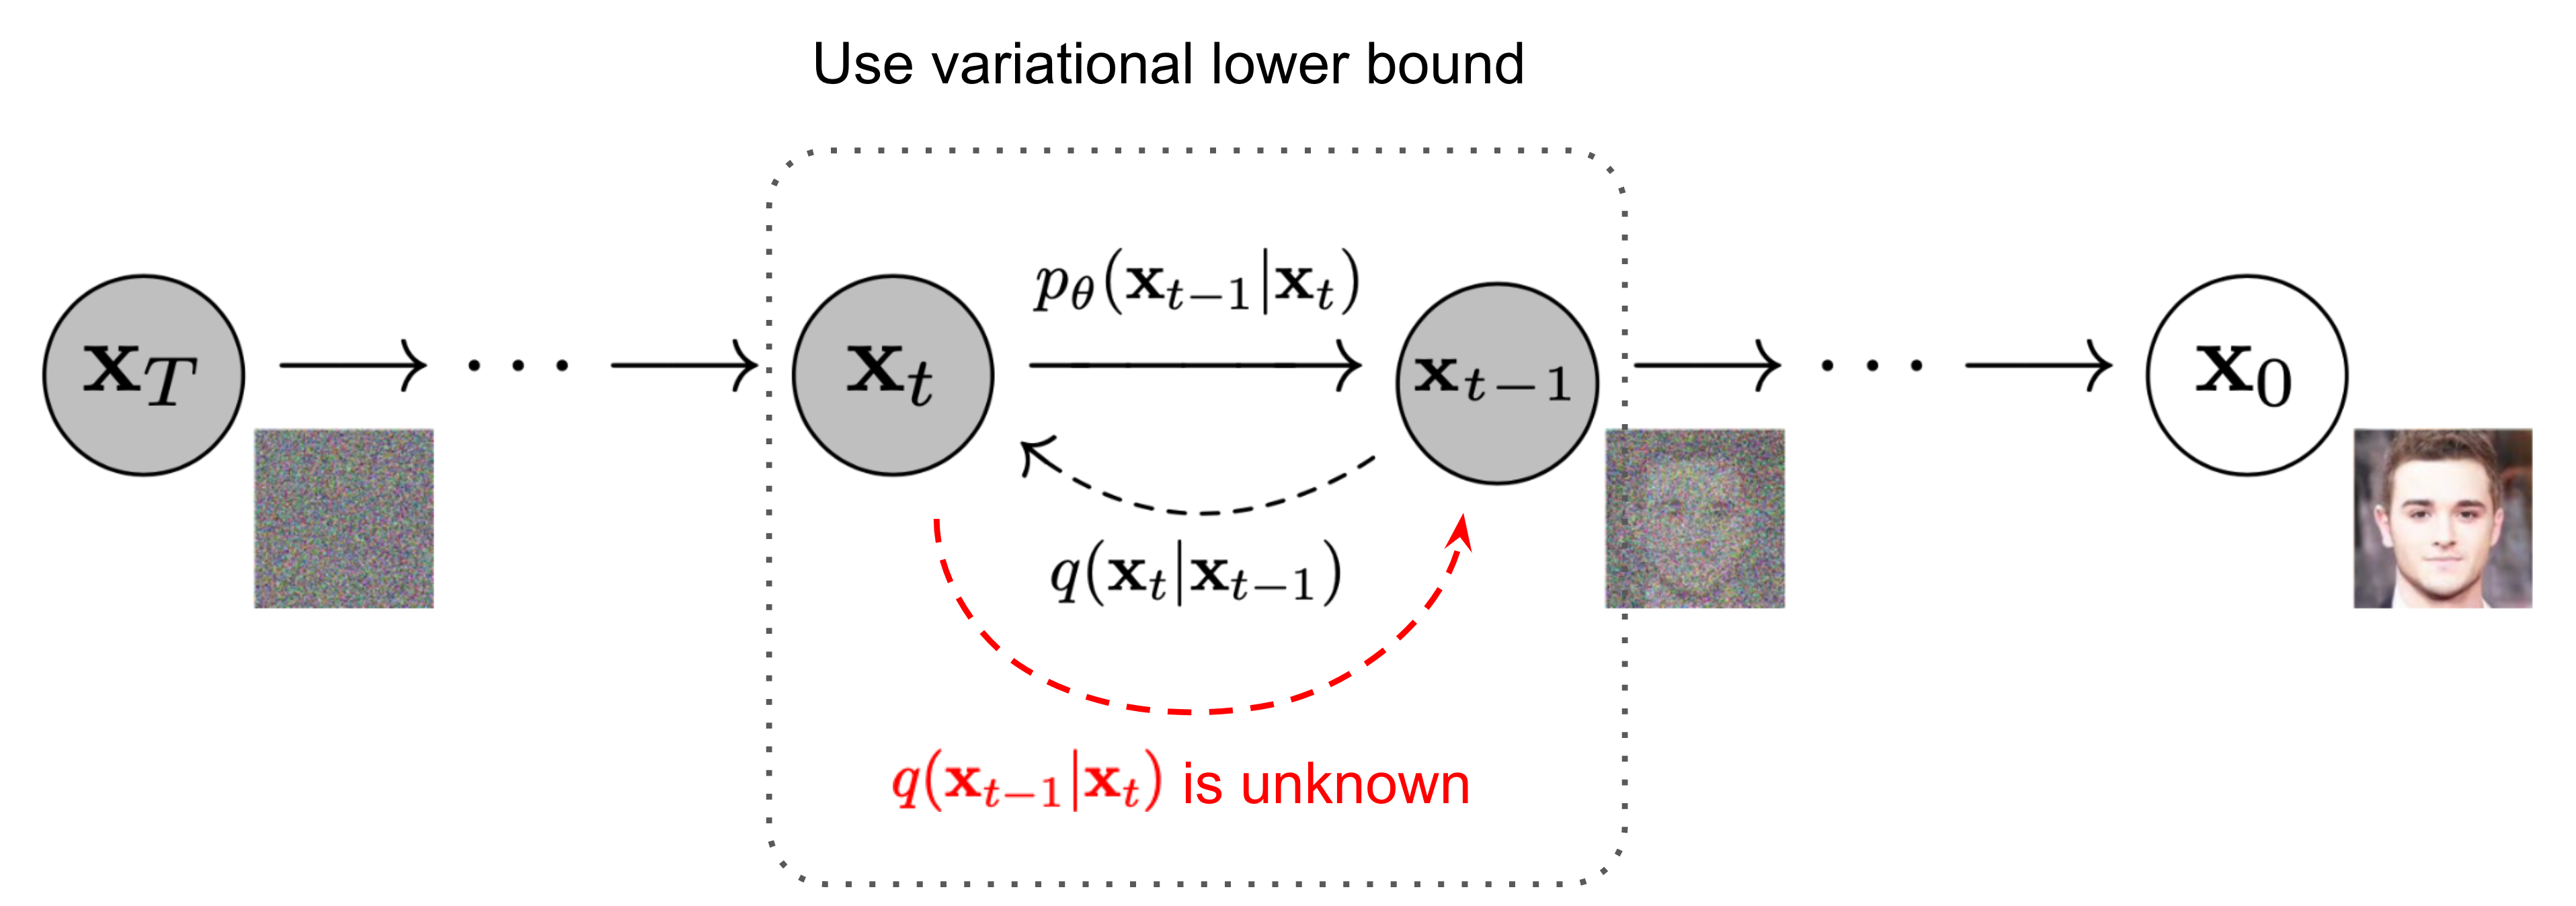
\includegraphics[width=0.9\linewidth]{concept_engineering/ddpm/DDPM.png}
    \caption{Visualization of the diffusion process\cite{ho2020denoisingdiffusionprobabilisticmodels}.}
    \label{fig:diffusion-process}
\end{figure}
Denoising Diffusion Probabilistic Models (DDPM)\cite{ho2020denoisingdiffusionprobabilisticmodels} are generative models that work by gradually adding noise to the data in several steps, and then learning how to reverse this process to recover the original data. The model learns to denoise the image step by step, starting from pure noise and progressively improving its reconstruction until it produces a realistic image. This approach allows DDPM to produce highly detailed synthetic images. 


\paragraph{Loss function}\mbox{}\\
\indent The loss function in DDPM is based on the evidence lower bound (ELBO\footnote{\url{https://en.wikipedia.org/wiki/Evidence_lower_bound}}), also known as "variational lower bound", which involves minimising the difference between the data distribution and the model distribution at each step of the diffusion process. In particular, it includes a term that encourages the model to effectively learn the backward diffusion process.

In practice, ELBO optimization is only the theoretical objective in DDPMs.
\textbf{M}ean \textbf{S}quared \textbf{E}rror and sometimes \textbf{A}bsolute \textbf{E}rror are the practical ways of loss calculation. They are used to calculate an error between added noise and predicted noise. The training objective is to minimize this error. This approach is an approximation of the ELBO optimization.\footnote{Full derivation can be seen in \cite{ho2020denoisingdiffusionprobabilisticmodels} or in this blogpost \url{https://learnopencv.com/denoising-diffusion-probabilistic-models/}}. 

% \begin{equation}
%     \centering
%     L(\theta)=\mathbb{E}_{t, x_0, \epsilon}\left[\left\|\epsilon-\epsilon_\theta\left(x_t, t\right)\right\|^2\right]
%     \label{loss-ddpm}
% \end{equation}

\begin{equation}
\begin{aligned} L_{\text {simple }}(\theta) & :=E_{t \sim U[1, T], \mathbf{x}_0, \epsilon}\left[\left\|\epsilon-\epsilon_\theta\left(\mathbf{x}_t, t\right)\right\|^2\right] \\ & =E_{t \sim U[1, T], \mathbf{x}_0, \epsilon}\left[\left\|\epsilon-\epsilon_\theta\left(\sqrt{\bar{\alpha}_t} \mathbf{x}_0+\sqrt{1-\bar{\alpha}_t} \epsilon, t\right)\right\|^2\right]
\end{aligned}
\end{equation}

where:
\begin{itemize}
    \item $x_0$ - original image,
    \item $T$ - number of timesteps, usually hundreds,
    \item $t$ - particular timestep,
    \item $\epsilon$ - gaussian noise added to original image,
    \item $\theta$ - neural network, for example U-Net,
    \item $\epsilon_\theta(x_t, t)$ - noise predicted by a neural network for a timestep $t$,
    \item $\overline{\alpha_t}$ - scaling factor,
\end{itemize}

The scaling factor is defined as cumulative product of all $\alpha$ between 1 and $t$. 
\begin{equation}
    \overline{\alpha_t} = \prod_{s=1}^t \alpha_s.
\end{equation}

\begin{equation}
    \alpha_t = 1-\beta_t
\end{equation}

The term $\beta_t$ is called "diffusion rate" for timestep $t$ and is calculated using a "noise scheduler". Such scheduler controls how much noise is added to an image in each step. Noise scheduler can be, for example, linear, scaled linear or squared cosine cap.

\paragraph{Training process}\mbox{}\\

\begin{figure}[H]
    \centering
    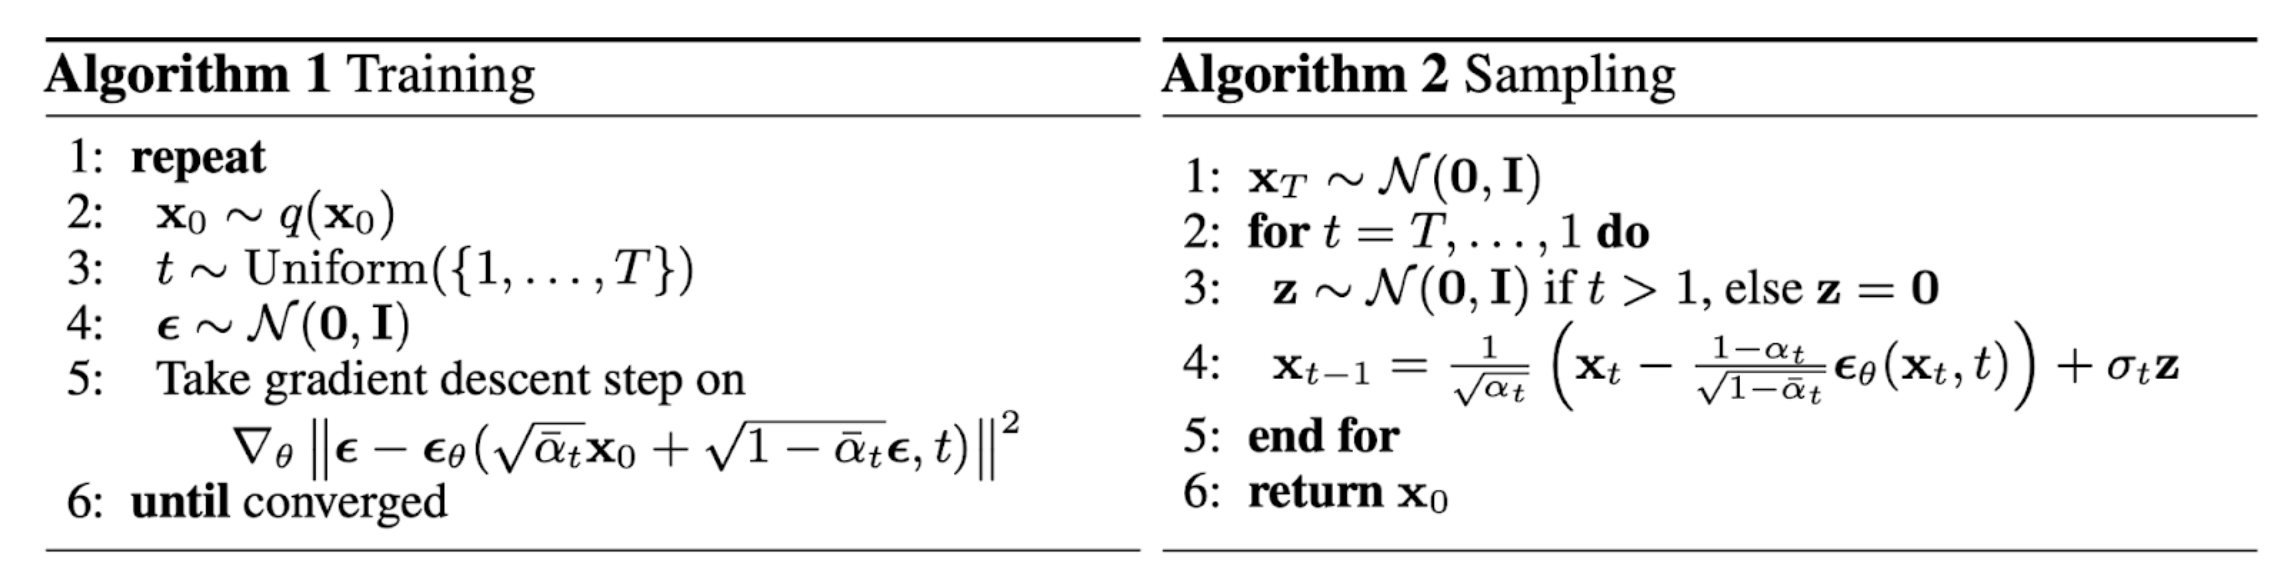
\includegraphics[width=0.9\linewidth]{concept_engineering/ddpm/DDPM-algo.png}
    \caption{Training and sampling algorithms for the diffusion process\cite{ho2020denoisingdiffusionprobabilisticmodels}.}
    \label{fig:diffusion-algo}
\end{figure}
In the training algorithm[\ref{fig:diffusion-algo}] the loss is calculated as a squared error between noise and predicted noise at a timestep $t$. However in practice all squared errors are calculated for each timestep $t$ and then final loss over an image (or a scan in 3D case) is calculated as a mean of these squared errors - MSE. 
This final loss is then aggregated with losses from the whole batch. In this point the gradient is calculated.  

\paragraph{Generation of CT scans}\mbox{}\\
\indent To generate artificial CT scans using DDPM, we could start by sampling gaussian noise and iteratively apply the learned reverse diffusion process. This process should refine the noise into a synthetic CT image that would progressively capture more and more of the anatomical details of the pelvis region.


\paragraph{Latent Diffusion Models}\mbox{}\\
\indent Latent diffusion models are diffusion models but in the latent space of an autoencoder. Unlike original diffusion, they do not generate an image from a Gaussian noise, but they generate its latent representation from a Gaussian noise. Then we can use a decoder to generate an image.
% \begin{figure}
%     \centering
%     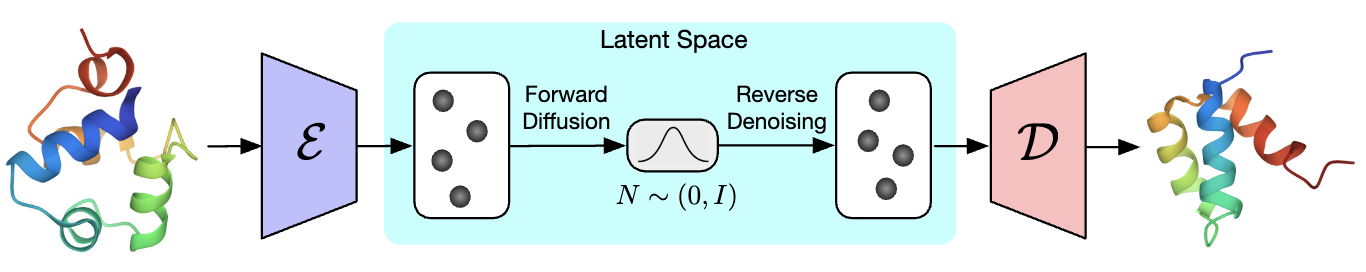
\includegraphics[width=\linewidth]{concept_engineering/ldm/LatentDiff.png}
%     \caption{Caption}
%     \label{fig:enter-label}
% \end{figure}

\begin{figure}[H]
    \centering
    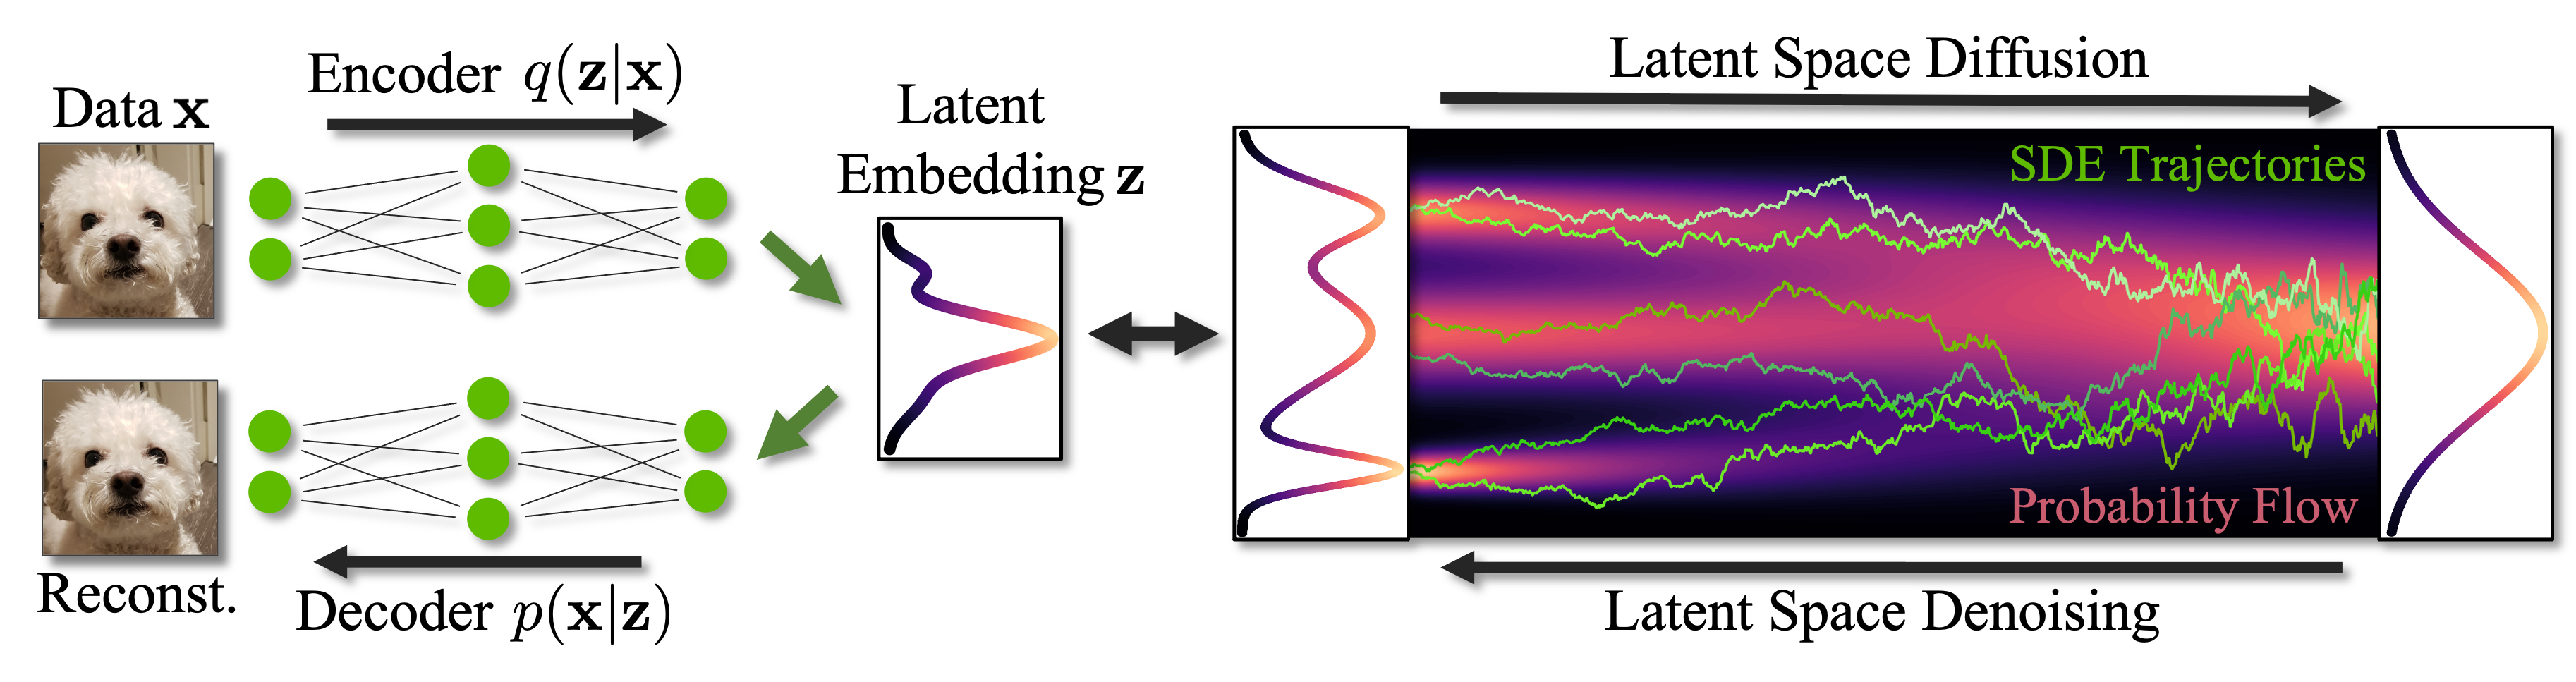
\includegraphics[width=\linewidth]{concept_engineering/ldm/ldm_figure.png}
    \caption{Visualization on how Latent Diffusion Models work. LDM learns latent representations distribution instead of distribution of input data\cite{neurips2023-ldm-tutorial/neurips2023-ldm-tutorial.github.io_2023}.}
    \label{fig:ldm}
\end{figure}

The idea of using diffusion model in the latent space will be used in the architectures below.
More information on LDM can be found on the website\footnote{\url{https://neurips2023-ldm-tutorial.github.io/}} and in the presentation\footnote{\url{https://drive.google.com/file/d/1p_aZ627Bwvku7nKyYRHtfZe50nAnpqGU/view}}.

\newpage
\subsubsection{VAE - Variational Autoencoder}
\begin{figure}[H]
    \centering
    \begin{tikzpicture}[
    box/.style={draw, minimum width=2cm, minimum height=3cm, text width=1.8cm, align=center},
    smallbox/.style={draw, minimum width=1.5cm, minimum height=1.2cm, text width=1.3cm, align=center},
    arrow/.style={->, >=latex, thick},
    label/.style={font=\small}
]

% Components
\node[circle, draw] (input) {Input $x$};
\node[box, right=1cm of input] (encoder) {Encoder};

% Latent space
\node[right=2cm of encoder] (latent) {};
\node[circle, draw, above=0.3cm of latent] (mu) {$\mu$};
\node[circle, draw, below=0.3cm of latent] (sigma) {$\sigma$};
\node[circle, draw, minimum size=1cm, right=1cm of latent] (z) {$z$};

\node[box, right=1cm of z] (decoder) {Decoder};
\node[circle, draw, right=1cm of decoder] (output) {Output $\hat{x}$};

% Reparameterization trick
\node[circle, draw, fill=white, minimum size=0.5cm, above=0.5cm of z] (epsilon) {$\epsilon$};

% Connections
\draw[arrow] (input) -- (encoder);
\draw[arrow] (encoder) -- (mu);
\draw[arrow] (encoder) -- (sigma);
\draw[arrow] (mu) -- (z);
\draw[arrow] (sigma) -- (z);
\draw[arrow] (epsilon) -- (z);
\draw[arrow] (z) -- (decoder);
\draw[arrow] (decoder) -- (output);

% Labels
\node[label, below=0.2cm of input] {High-dimensional};
% \node[label, above=0.2cm of mu] {Latent space};
\node[label, below=0.2cm of sigma] {Latent space};
\node[label, above=0.2cm of epsilon] {$\sim \mathcal{N}(0,1)$};
\node[label, below=0.2cm of output] {Reconstructed};

% % KL Divergence
% \draw[<->, >=latex, bend left=30] ($(encoder.north east)+(0.2,0.2)$) to node[above, font=\small] {KL Divergence} ($(mu.north west)+(-0.2,0.2)$);

% Reconstruction Loss
\draw[<->, >=latex, bend right=30] ($(input.south west)+(1,-0.3)$) to node[below, font=\small] {Reconstruction Loss} ($(output.south east)+(-1.3,-0.2)$);

\end{tikzpicture}
    \caption{Visualization of Variational Autoencoder. Circles are tensors, rectangles are neural networks.}
    \label{fig:vae}
\end{figure}

\indent The main issue with autoencoders in the context of synthetic data generation is that we do not know what values should be assigned to the layer $z$ and passed through decoder in order to obtain meaningful results. The Variational Autoencoder addresses it.
This model extends the standard autoencoder by linking it with probability concepts: mean and standard deviation. VAE learns not only to create a compressed representation of the data, but also a distribution over that representation. This makes VAEs capable of generating new data samples that are similar to those in the training set. Thus, VAE is a suitable choice for image generation, data augmentation, and even anomaly detection.

\begin{figure}[H]
    \centering
    
\begin{tikzpicture}[
    neuron/.style={circle, draw, minimum size=0.5cm},
    layer/.style={rectangle, draw, rounded corners, minimum height=3cm, minimum width=1cm, fill opacity=0.2},
    arrow/.style={->, >=latex, thick},
    label/.style={font=\small}
]

% Color definitions
\colorlet{input}{gray!20}
\colorlet{encoder}{blue!40}
\colorlet{mu}{orange!20}
\colorlet{sigma}{blue!20}
\colorlet{latent}{green!20}
\colorlet{decoder}{red!20}

% Input layer
\node[layer, fill=input] (input) {};
\foreach \y in {1,...,4} {
    \node[neuron, fill=input] (i\y) at (input.west |- input.north) [yshift=-\y*0.60cm, xshift=0.5cm] {};
}

% Encoder layer
\node[layer, fill=encoder, right=1.5cm of input] (encoder) {};
\foreach \y in {1,...,3} {
    \node[neuron, fill=encoder] (e\y) at (encoder.west |- encoder.north) [yshift=-\y*0.8cm, xshift=0.5cm] {};
}

% Mu layer
\node[layer, fill=mu, right=1.5cm of encoder, minimum height=1.5cm, yshift=0.75cm] (mu) {};
\foreach \y in {1,...,2} {
    \node[neuron, fill=mu] (mu\y) at (mu.west |- mu.north) [yshift=-\y*0.5cm, xshift=0.5cm] {};
}

% Sigma layer
\node[layer, fill=sigma, below=0.5cm of mu, minimum height=1.5cm] (sigma) {};
\foreach \y in {1,...,2} {
    \node[neuron, fill=sigma] (sigma\y) at (sigma.west |- sigma.north) [yshift=-\y*0.5cm, xshift=0.5cm] {};
}

% Latent layer
\node[layer, fill=latent, right=1.5cm of mu, yshift=-0.75cm, minimum height=2cm] (latent) {};
\foreach \y in {1,...,2} {
    \node[neuron, fill=latent] (l\y) at (latent.west |- latent.north) [yshift=-\y*0.7cm, xshift=0.5cm] {};
}

% Decoder layer
\node[layer, fill=decoder, right=1.5cm of latent] (decoder) {};
\foreach \y in {1,...,3} {
    \node[neuron, fill=decoder] (d\y) at (decoder.west |- decoder.north) [yshift=-\y*0.7cm, xshift=0.5cm] {};
}

% Output layer
\node[layer, fill=input, right=1.5cm of decoder] (output) {};
\foreach \y in {1,...,4} {
    \node[neuron, fill=input] (o\y) at (output.west |- output.north) [yshift=-\y*0.65cm, xshift=0.5cm] {};
}

% Connections
\foreach \i in {1,...,4} {
    \foreach \j in {1,...,3} {
        \draw[blue!50, thick] (i\i) -- (e\j);
    }
}

\foreach \i in {1,...,3} {
    \foreach \j in {1,...,2} {
        \draw[orange!50, thick] (e\i) -- (mu\j);
        \draw[blue!50, thick] (e\i) -- (sigma\j);
    }
}

\foreach \i in {1,...,2} {
    \draw[green!50, thick] (mu\i) -- (l\i);
    \draw[green!50, thick] (sigma\i) -- (l\i);
}

\foreach \i in {1,...,2} {
    \foreach \j in {1,...,3} {
        \draw[red!50, thick] (l\i) -- (d\j);
    }
}

\foreach \i in {1,...,3} {
    \foreach \j in {1,...,4} {
        \draw[red!50, thick] (d\i) -- (o\j);
    }
}

% Labels
\node[label, above=0.2cm of input] {$x$};
\node[label, above=0.2cm of encoder] {$E$};
\node[label, above=0.2cm of mu] {$\mu(x)$};
\node[label, below=0.2cm of sigma] {$\sigma(x)$};
\node[label, above=0.2cm of latent] {$z \sim \mathcal{N}(\mu, \sigma)$};
\node[label, above=0.2cm of decoder] {$D$};
\node[label, above=0.2cm of output] {$\hat{x} = D(z)$};

\end{tikzpicture}
    \caption{Visualization of a simple VAE.}
    \label{fig:vae-simple}
\end{figure}

The figure[\ref{fig:vae-simple}] shows detailed visualization of a simple Variational Autoencoder. It is worth noticing that the encoder $E$ has two outputs, $\mu$ and $\sigma$, which produce $z$ using the reparameterization trick\footnote{\url{https://www.baeldung.com/cs/vae-reparameterization}}.

\begin{equation}
    z = \mu + \sigma\cdot\epsilon,
\end{equation}

where $\epsilon\sim\mathcal{N}(0,1)$.

\paragraph{Loss Function:}\mbox{}\\
The VAE loss is a combination of:
\begin{enumerate}
\item \textbf{Reconstruction Loss}, which ensures how well the reconstructed image matches the original input image, for example $L1$, $L2$, $MSE$,
\item \textbf{KL Divergence Loss} that ensures the latent space follows a Gaussian distribution.
\end{enumerate}

\begin{equation}
    L = L_{reconstruction} + \mathbb{KL}(q(z | x) || p(z)),
\end{equation}

where 
\begin{itemize}
    \item $\mathbb{KL}$ - Kullback-Leibler divergence\footnote{\url{https://en.wikipedia.org/wiki/Kullback\%E2\%80\%93Leibler_divergence}}, measures how much two distributions differ from each other,
    \item $q(z | x) = \mathcal{N}(\mu, \sigma)$ - probability distribution of the latent representation $z$, in other words probability distribution of endocers output,
    \item $p(z) = \mathcal{N}(0,1)$ - expected probability distribution.
\end{itemize}

After substituting probabilities, the loss $L$ becomes\footnote{Broader explanation and Pytorch toy example can be found here \url{https://avandekleut.github.io/vae/}.}
\begin{equation}
    L = L_{reconstruction} + \mathbb{KL}(\mathcal{N}(\mu,\sigma), \mathcal{N}(0,1)).
\end{equation}

The difference between two Gaussians can be calculated using the identity\cite{7449}. 

\begin{equation}
    \mathbb{KL}\left( \mathcal{N}(\mu, \sigma) \parallel \mathcal{N}(0, 1) \right) = \sum_{x \in X} \left( \sigma^2 + \mu^2 - \log \sigma - \frac{1}{2} \right)
\end{equation}


% Train the VAE on prostate CT scans to learn an efficient latent space representation.
\paragraph{Generation of CT scans}\mbox{}\\

To generate new CT scans, we could sample the Gaussian noise tensor of shape $z$, which follows the normal distribution, and then pass it through the decoder.
If the model is properly trained, the decoder should reconstruct this latent representation into a realistic synthetic CT image. 

However, it is not guaranteed that the learned distribution $q(z)$ is always similar to $\mathbf{N}(0,1)$, especially when the $\mathbb{KL}$ loss is far from $0$. To mitigate this issue, aggregated posterior probability could be used. For example, by passing the entire dataset through the encoder and averaging resulted in $\mu$s to $\overline{\mu}$ and $\sigma$s to $\overline{\sigma}$ and then sampling from $\mathcal{N}(\overline{\mu}, \overline{\sigma})$. The alternative solution is to train another neural network that would learn the distribution of the latent representation of $z$ - $q(z)$. Such a neural network could be a Latent Diffusion Model described in the previous section.

% ### Key Differences from Traditional Autoencoders

% ### VAE Structure

% 1. **Encoder (Inference Network)**: The encoder maps an input \( x \) to a latent representation, but instead of outputting a single value, it outputs parameters of a probability distribution, typically a Gaussian distribution with a mean \( \mu \) and a variance \( \sigma^2 \). This is achieved by splitting the encoder's output into two parts:

% \[
% q(z|x) = \mathcal{N}(z; \mu(x), \sigma^2(x))
% \]

% where:
% - \( \mu(x) \) is the mean of the latent distribution for input \( x \),
% - \( \sigma^2(x) \) is the variance of the latent distribution for input \( x \),
% - \( z \) is the latent variable sampled from the distribution \( q(z|x) \).

% 2. **Reparameterization Trick**: To allow backpropagation through the stochastic sampling process, VAEs use the reparameterization trick. Instead of sampling \( z \) directly from \( \mathcal{N}(\mu(x), \sigma^2(x)) \), a random variable \( \epsilon \sim \mathcal{N}(0, 1) \) is sampled, and \( z \) is computed as:

% \[
% z = \mu(x) + \sigma(x) \cdot \epsilon
% \]

% This trick makes the sampling process differentiable, enabling gradient-based optimization.

% 3. **Decoder (Generative Network)**: The decoder reconstructs the input data from the latent variable \( z \). The decoder maps \( z \) back to the data space, producing a reconstruction \( \hat{x} \). Similar to traditional autoencoders, this is done through a neural network.

% ### VAE Loss Function

% The loss function in a VAE consists of two terms:

% 1. **Reconstruction Loss**: This measures how well the decoder can reconstruct the input from the latent variable \( z \). It is typically the Mean Squared Error (MSE) or binary cross-entropy, depending on the nature of the data:

% \[
% L_{reconstruction} = \mathbb{E}_{q(z|x)} [||x - \hat{x}||^2]
% \]

% 2. **KL Divergence (Regularization Term)**: The second term ensures that the learned latent distribution \( q(z|x) \) is close to a chosen prior distribution \( p(z) \) (usually a standard normal distribution \( \mathcal{N}(0, 1) \)). This regularization term is the Kullback-Leibler (KL) divergence between the approximate posterior \( q(z|x) \) and the prior \( p(z) \):

% \[
% D_{KL}(q(z|x) || p(z)) = \frac{1}{2} \sum_{i=1}^n (1 + \log(\sigma_i^2) - \mu_i^2 - \sigma_i^2)
% \]

% The total VAE loss is a combination of the reconstruction loss and the KL divergence:

% \[
% L_{VAE} = L_{reconstruction} + D_{KL}(q(z|x) || p(z))
% \]

% This loss encourages the model to reconstruct the input data accurately while ensuring that the latent variables follow the prior distribution.

% ### Applications

% 1. **Data Generation**: By sampling latent vectors from the learned distribution, VAEs can generate new data points similar to those in the training set.
   
% 2. **Anomaly Detection**: VAEs can detect anomalies by measuring the reconstruction error for unseen data; higher reconstruction errors often indicate anomalies.
   
% 3. **Data Augmentation**: VAEs can be used to generate additional synthetic data for training, improving model generalization.

% 4. **Latent Space Exploration**: The continuous and smooth latent space learned by VAEs allows for meaningful interpolations between data points.

% ---

% **References**:
% 1. Kingma, D. P., & Welling, M. (2013). *Auto-Encoding Variational Bayes*. arXiv preprint arXiv:1312.6114.
% 2. Doersch, C. (2016). *Tutorial on Variational Autoencoders*. arXiv preprint arXiv:1606.05908.
% \begin{tikzpicture}[
    box/.style={draw, minimum width=2cm, minimum height=3cm, text width=1.8cm, align=center},
    smallbox/.style={draw, minimum width=1.5cm, minimum height=1.2cm, text width=1.3cm, align=center},
    arrow/.style={->, >=latex, thick},
    label/.style={font=\small}
]

% Components
\node[circle, draw] (input) {Input $x$};
\node[box, right=1cm of input] (encoder) {Encoder};

% Latent space
\node[right=2cm of encoder] (latent) {};
\node[circle, draw, above=0.3cm of latent] (mu) {$\mu$};
\node[circle, draw, below=0.3cm of latent] (sigma) {$\sigma$};
\node[circle, draw, minimum size=1cm, right=1cm of latent] (z) {$z$};

\node[box, right=1cm of z] (decoder) {Decoder};
\node[circle, draw, right=1cm of decoder] (output) {Output $\hat{x}$};

% Reparameterization trick
\node[circle, draw, fill=white, minimum size=0.5cm, above=0.5cm of z] (epsilon) {$\epsilon$};

% Connections
\draw[arrow] (input) -- (encoder);
\draw[arrow] (encoder) -- (mu);
\draw[arrow] (encoder) -- (sigma);
\draw[arrow] (mu) -- (z);
\draw[arrow] (sigma) -- (z);
\draw[arrow] (epsilon) -- (z);
\draw[arrow] (z) -- (decoder);
\draw[arrow] (decoder) -- (output);

% Labels
\node[label, below=0.2cm of input] {High-dimensional};
% \node[label, above=0.2cm of mu] {Latent space};
\node[label, below=0.2cm of sigma] {Latent space};
\node[label, above=0.2cm of epsilon] {$\sim \mathcal{N}(0,1)$};
\node[label, below=0.2cm of output] {Reconstructed};

% % KL Divergence
% \draw[<->, >=latex, bend left=30] ($(encoder.north east)+(0.2,0.2)$) to node[above, font=\small] {KL Divergence} ($(mu.north west)+(-0.2,0.2)$);

% Reconstruction Loss
\draw[<->, >=latex, bend right=30] ($(input.south west)+(1,-0.3)$) to node[below, font=\small] {Reconstruction Loss} ($(output.south east)+(-1.3,-0.2)$);

\end{tikzpicture}
% Reparametrization trick


% \begin{tikzpicture}[
    node distance = 1cm and 2cm,
    every node/.style = {draw, minimum size=0.8cm},
    % square/.style = {sides=4},
    square/.style = {regular polygon,regular polygon sides=4},
    arr/.style = {->, >=stealth}
]

% Original graph
\node[square] (f1) at (0,0) {$f$};
\node[circle] (z1) at (0,-1.5) {$z$};
\node[square] (mu1) at (-1,-3) {$\mu$};
\node[square] (sigma1) at (1,-3) {$\sigma$};

\draw[arr] (mu1) -- (z1);
\draw[arr] (sigma1) -- (z1);
\draw[arr] (z1) -- (f1);

\node[below=0.5cm of sigma1, draw=none] {Original};

% Reparametrized graph
\node[square] (f2) at (5,0) {$f$};
\node[square] (z2) at (5,-1.5) {$z$};
\node[square] (mu2) at (4,-3) {$\mu$};
\node[square] (sigma2) at (5,-3) {$\sigma$};
\node[circle] (epsilon) at (6,-3) {$\varepsilon$};

\draw[arr] (mu2) -- (z2);
\draw[arr] (sigma2) -- (z2);
\draw[arr] (epsilon) -- (z2);
\draw[arr] (z2) -- (f2);

\node[below=0.5cm of sigma2, draw=none] {Reparametrized};

\end{tikzpicture}

\newpage
\subsubsection{VQVAE}
% \begin{tikzpicture}[
    box/.style={draw, minimum width=2cm, minimum height=3cm, text width=1.8cm, align=center},
    smallbox/.style={draw, minimum width=1.5cm, minimum height=1.2cm, text width=1.8cm, align=center},
    arrow/.style={->, >=latex, thick},
    label/.style={font=\small},
    % circle/.style={draw, align=center}
]

% Components
\node[circle, draw] (input) {Input $x$};
\node[box, right=1cm of input] (encoder) {Encoder};

% Latent space
\node[right=2cm of encoder] (latent) {};
\node[circle, draw, right=1cm of encoder, font=\small, align=center,text width=2cm] (quantized) {Quantized \\ z};
\node[smallbox, below=0.3cm of quantized] (codebook) {Codebook};

\node[box, right=2cm of latent] (decoder) {Decoder};
\node[circle, draw, right=1cm of decoder] (output) {Output $\hat{x}$};

% Connections
\draw[arrow] (input) -- (encoder);
\draw[arrow] (encoder) -- (quantized);
\draw[arrow] (codebook) -- (quantized);
\draw[arrow] (quantized) -- (decoder);
\draw[arrow] (decoder) -- (output);

% Labels
\node[label, below=0.2cm of input] {High-dimensional};
\node[label, below=0.2cm of codebook] {Latent space};
\node[label, below=0.2cm of output] {Reconstructed};

% Reconstruction Loss
\draw[<->, >=latex, bend right=30] ($(input.south west)+(1,-0.3)$) to node[below, font=\small] {Reconstruction Loss} ($(output.south east)+(-1.3,-0.2)$);

% Commitment Loss
\draw[<->, >=latex, bend left=40] ($(encoder.north east)+(0.2,0.2)$) to node[above=0.1cm, font=\small] {Commitment Loss} ($(quantized.north west)+(-0.2,0.2)$);

\end{tikzpicture}
\begin{figure}[H]
    \centering
    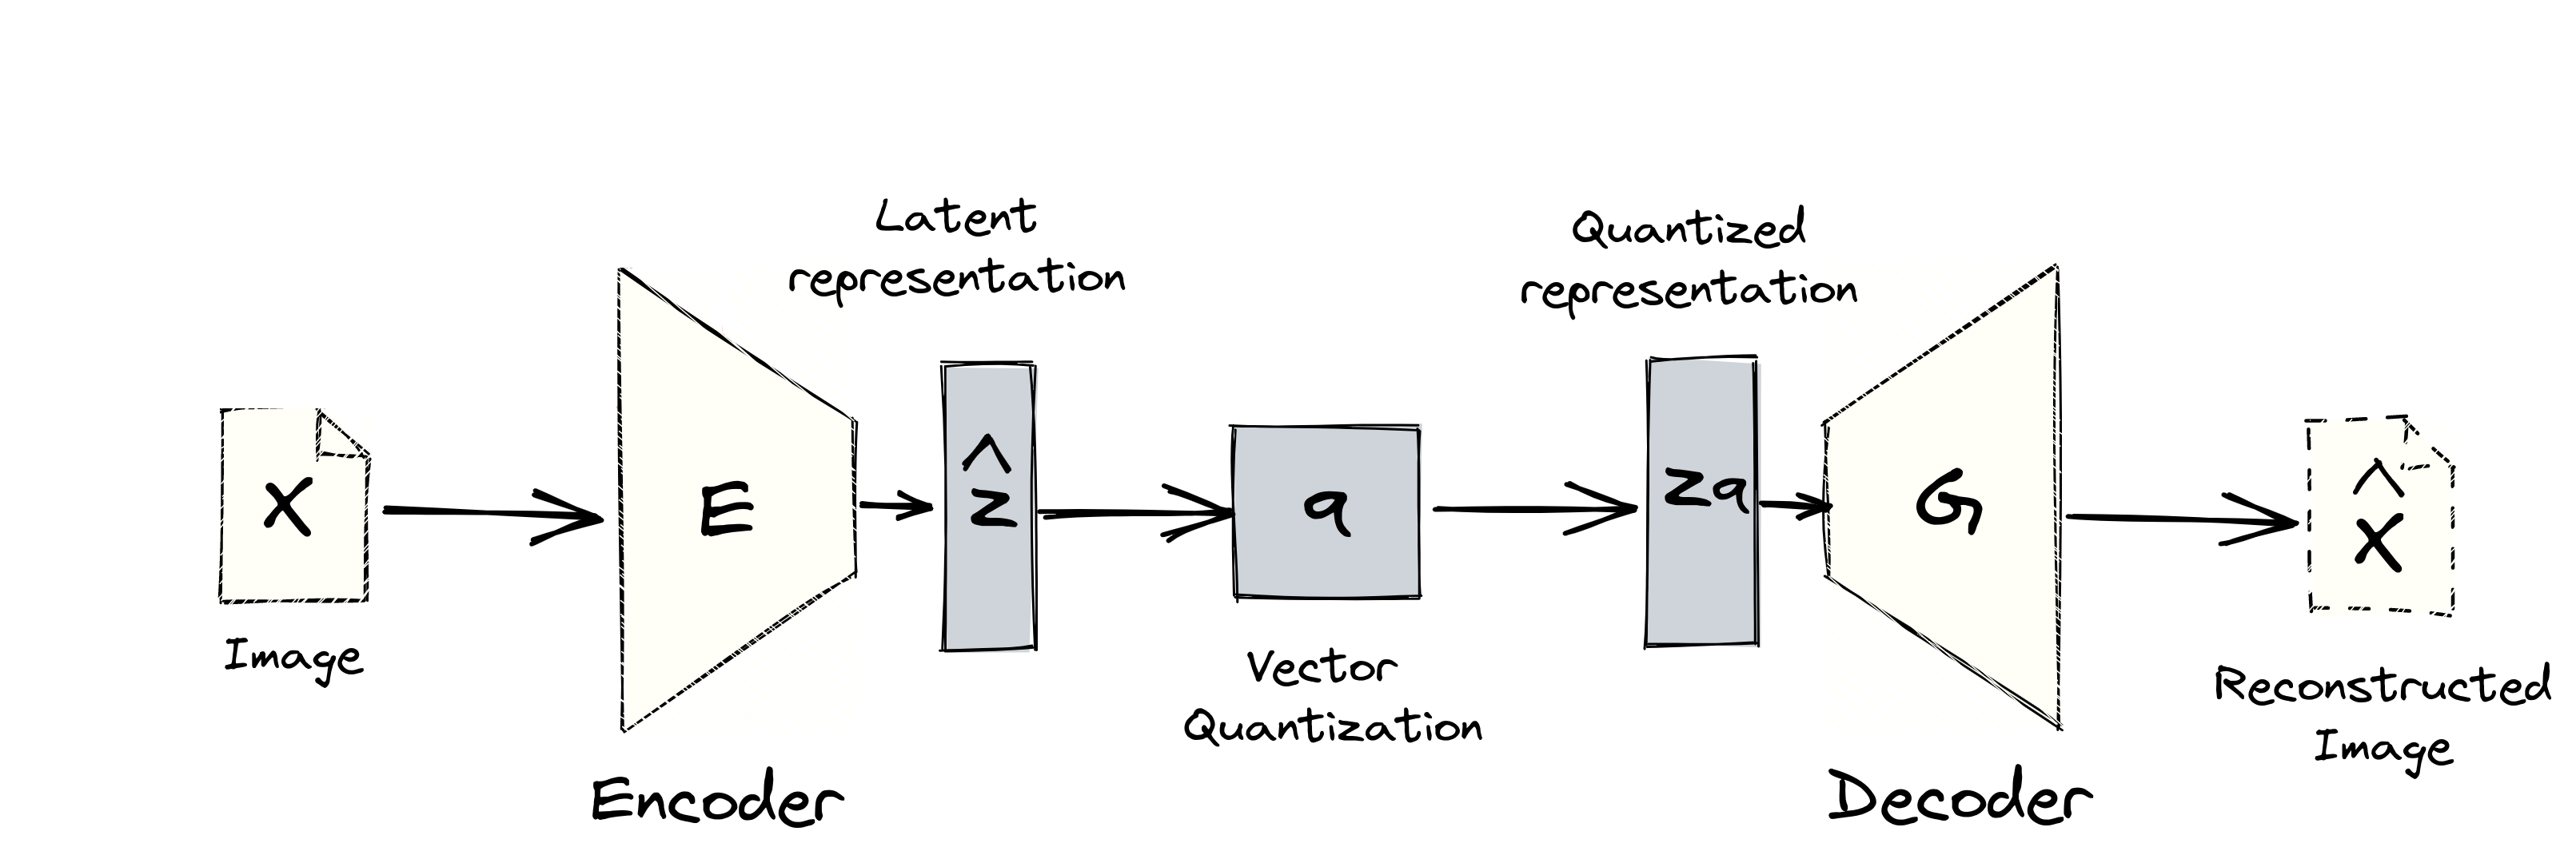
\includegraphics[width=\linewidth]{concept_engineering/vqgan/vqvae.png}
    \caption{Visualization of Vector Quantized Variational Autoencoder\cite{miranda2021vqgan}.}
    \label{fig:vavae1}
\end{figure}

The variational autoencoders latent representation $z$ can have any value, usually from the distribution $\sim \mathbb{N}(0,1)$. Unfortunately, it sometimes leads to posterior collapse. This means that the decoder starts to treat latent representation $z$ as meaningless noise and ignores it. Instead, it learns to encode the dataset in itself. When something like this happens decoder cannot generate meaningful results, no matter the given $z$. 

\begin{figure}[H]
    \centering
    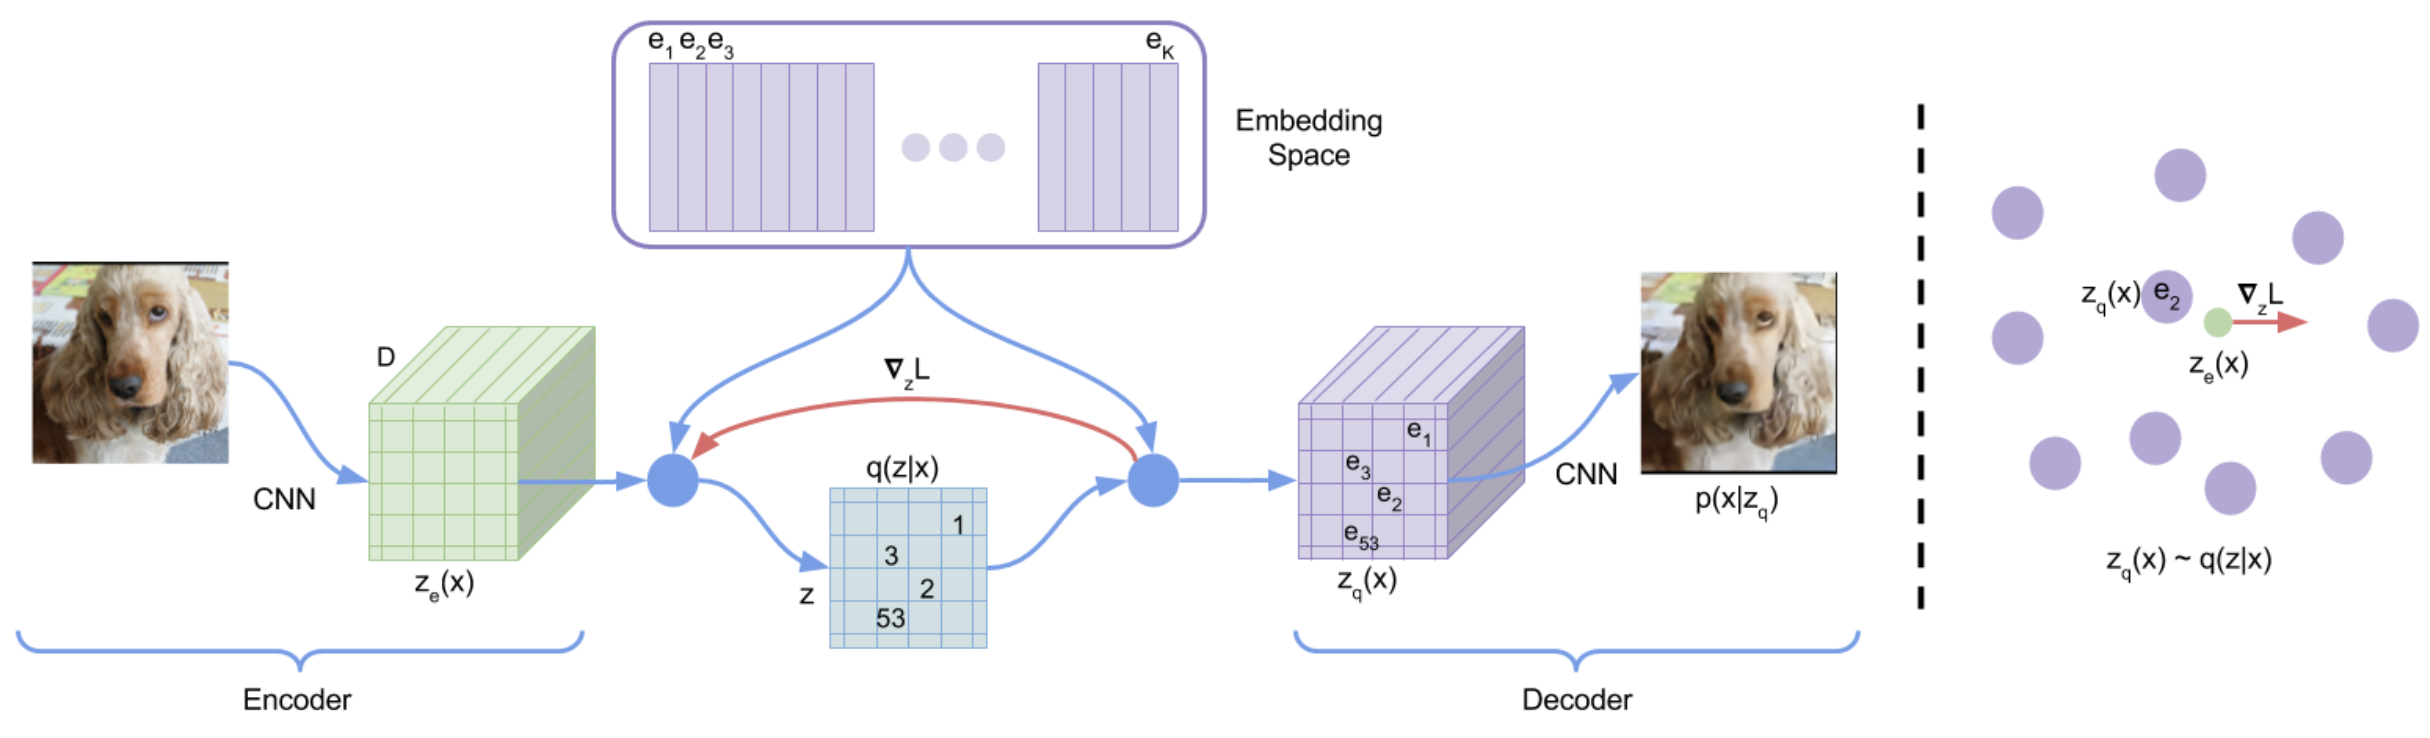
\includegraphics[width=\linewidth]{concept_engineering/vqvae.png}
    \caption{VQVAE visualization showing compression of an image to latent representation (a cube), encoding and decompression\cite{oord2018neuraldiscreterepresentationlearning}.}
    \label{fig:vqvae-paper}
\end{figure}

To mitigate this issue, researchers\cite{oord2018neuraldiscreterepresentationlearning} came up with the idea of having a fixed set of latent representations that hold semantic meaning. In case of images, the encoder compresses the original image of dimensions $(C,H,W)$ to its latent representation $(D,H_2,W_2)$ (a tensor "cube"), where $C<D$, $H>H_2$ and $W>W_2$. Then each latent "pixel" (a cell on a figure\ref{fig:vqvae-paper}) gets a vector from the codebook that holds the semantic meaning of this part of the compressed image. 

%the image to codes from the codebook and then uses the decoder to retrieve the original value. 

\paragraph{Loss function}\mbox{}\\
% Reconstruction Loss (between input and output) and Commitment Loss (penalizing the difference between encoder outputs and quantized embeddings).
The VQVAE loss has three parts.

\begin{itemize}
    \item \textbf{Reconstruction loss} the same as in the VAE, measures how ensures the output matches the input.
    \item \textbf{Commitment loss} - penalizes the difference between encoder outputs and quantized embeddings,
    \item \textbf{Codebook loss} - it is the same value as commitment loss, however it is used to change values of codebook representations through backpropagation.
\end{itemize}

which can be expressed by this formula
\begin{equation}
    L_{VQ}(E, G, Z) = \underbrace{||x-\hat{x}||^{2}}_{\text{reconstruction loss}} + \underbrace{||sg[E(x)] - z_\mathbf{q}||_2^2}_{\text{codebook loss}}
+ \underbrace{||sg[z_\mathbf{q}] - E(x) ||_{2}^2}_{\text{commitment loss}},
    \label{loss_vq}
\end{equation}

where
\begin{itemize}
    \item $\hat{x}$ - reconstructed image,
    \item $E(x)=\hat{z}$ - encoder output,
    \item $z_\mathbf{q}$ - quantized $\hat{z}$,
    \item $sg$ - stop gradient.
\end{itemize}

VQVAE models have one important metric to note - Perplexity. It measures utilization of the codebook during embeeding. Higher is better.

% Codebook Loss: Ensures the quantized latent vectors match the encoder output.
% The commitment loss encourages the encoder to use the codebook efficiently.
\paragraph{Generation of CT scans}\mbox{}\\
\indent Unlike in case of VAE, the probability distribution $q(z_e|x)$ is not conditioned to be close to $\mathcal{N}(0,1)$. Thus, to generate a new image, one cannot just pass a Gaussian noise tensor through the codebook and decoder.
Instead, after successful training of VQVAE, another model like LDM should be used to learn to generate $z_e$ from Gaussian noise.

After that, to generate a synthetic CT scan, one can generate a tensor $z$ of Gaussian noise and then pass it through the denoising LDM to obtain $z_e$. Next, the closest codebook vector should be chosen for each "hidden pixel", for example using L1, L2 or MSE. After that, one would obtain $z_q$, which should then pass through the decoder to obtain the synthetic image.


% should be created and used to select the closest latent code from the codebook. Then the retrieved latent code should be passed through the decoder in order to transform it into a synthetic CT image.

% The target is to:
% $$ (\phi,\theta)=\underset{\phi,\theta}{\mathrm{argmax}}\quad\sum_{\mathbf{x}\in\mathcal{X}}\mathrm{ELBO}(\mathbf{x}), $$

% $$ \begin{aligned}\nabla_{\boldsymbol{\theta},\boldsymbol{\phi}}\:\mathrm{ELBO}(\mathbf{x}) & =\nabla_{\boldsymbol{\theta},\boldsymbol{\phi}}\left\{\mathbb{E}_{q_{\phi}(\mathbf{z}|\mathbf{x})}\left[\log\frac{p_{\boldsymbol{\theta}}(\mathbf{x},\mathbf{z})}{q_{\boldsymbol{\phi}}(\mathbf{z}|\mathbf{x})}\right]\right\}\\  & =\nabla_{\boldsymbol{\theta},\boldsymbol{\phi}}\Big{\{}\mathbb{E}_{q_{\mathrm{o}}(\mathbf{z}|\mathbf{x})}\Big{[}\log p_{\boldsymbol{\theta}}(\mathbf{x},\mathbf{z})-\log q_{\boldsymbol{\phi}}(\mathbf{z}|\mathbf{x})\Big{]}\Big{\}}.\end{aligned} $$

% $$ (\boldsymbol{\mu},\boldsymbol{\sigma}^2)=\mathrm{EncoderNetwork}_{\boldsymbol{\phi}}(\mathbf{x})\\q_{\phi}(\mathbf{z}|\mathbf{x})=\mathcal{N}(\mathbf{z}\mid\boldsymbol{\mu},\mathrm{diag}(\boldsymbol{\sigma}^2)) $$

% $$ (\boldsymbol{\mu},\sigma^2)=\mathrm{EncoderNetwork}_{\boldsymbol{\phi}}(\mathbf{x})q_{\phi}(\mathbf{z}|\mathbf{x})=\mathcal{N}(\mathbf{z}\mid\mathbf{\mu},\sigma^2\mathbf{I} $$

% $$ \begin{aligned}\mu & =\underbrace{\mu_{\phi}}_{\text{neural network}}(\mathbf{x}),\\ \sigma^2 & =\underbrace{\sigma_{\phi}^2}_{\text{neural network}}(\mathbf{x}),\end{aligned} $$


% $$ \begin{aligned}\mathrm{ELBO}_{\boldsymbol{\phi},\boldsymbol{\theta}}(\mathbf{x}) & =\mathbb{E}_{q_{\boldsymbol{\phi}}(\mathbf{x}_1|\mathbf{x}_0)}\Big{[}\log\underbrace{p_{\boldsymbol{\theta}}(\mathbf{x}_0|\mathbf{x}_1)}_{\mathrm{how~good~the~tintial~block~is}}\Big{]}\\  & -\mathbb{E}_{q_{\boldsymbol{\phi}}(\mathbf{x}_{T-1}|\mathbf{x}_0)}\Big{[}\underbrace{\mathbb{D}_{\mathrm{KL}}\Big{(}q_{\boldsymbol{\phi}}(\mathbf{x}_{T}|\mathbf{x}_{T-1})\|p(\mathbf{x}_{T})\Big{)}\Big{]}}_{\mathrm{how~good~the~final~block~is}}\Big{]}\\  & -\sum_{t=1}^{T-1}\mathbb{E}_{q_{\boldsymbol{\theta}}(\mathbf{x}_{t-1},\mathbf{x}_{t+1}|\mathbf{x}_0)}\Big{[}\underbrace{\mathbb{D}_{\mathrm{KL}}\Big{(}q_{\boldsymbol{\phi}}(\mathbf{x}_{t}|\mathbf{x}_{t-1})\|p_{\boldsymbol{\theta}}(\mathbf{x}_{t}|\mathbf{x}_{t+1})\Big{)}}_{\mathrm{how~good~the~transition~blocks~are}}\Big{]},\end{aligned} $$

\newpage
\subsubsection{VQGAN} 
VQGAN proposed in \cite{Esser_2021_CVPR} is a hybrid model that combines VQVAE's structured latent space with GANs. VQGAN can create high-quality images by using GANs to make textures and details look more realistic.
% This technique, in comparison to the direct use of diffusion models to 3D data, allows one to train a model using less computational resources and sampling from compressed latent space that has an abstract representation of the input.

\begin{figure}[H]
    \centering
    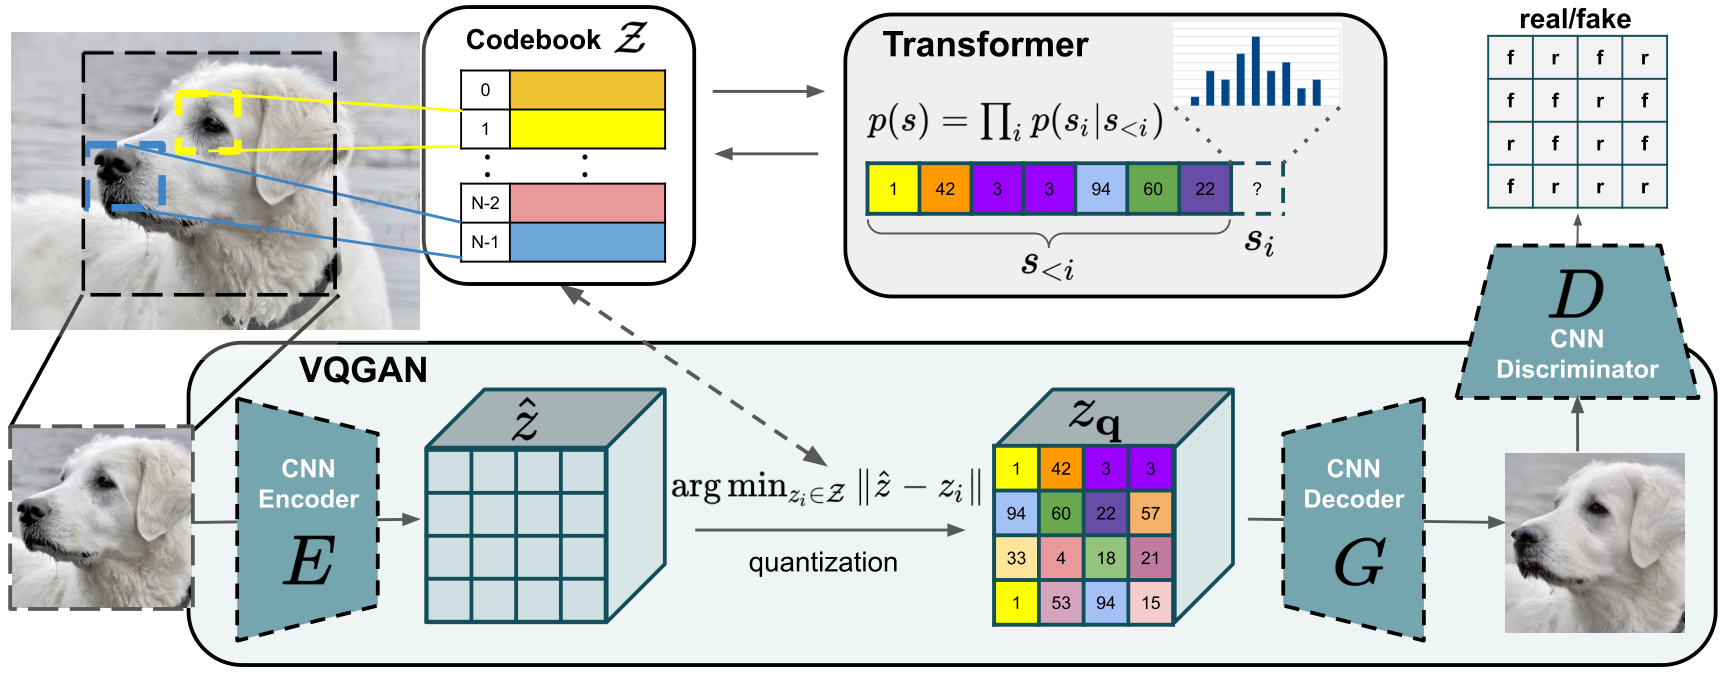
\includegraphics[width=0.9\linewidth]{concept_engineering/vqgan/vqgan.png}
    \caption{VQGAN visualization.\cite{Esser_2021_CVPR}. }
    \label{fig:vqgan-diagram}
\end{figure}

VQGAN has also a transformer part, which is trained to learn connections between embeeding vectors. It is useful for generating images from text.
\paragraph{Loss function}\mbox{}\\

The loss function for VQGAN combines VQVAE and GAN losses:

\begin{itemize}
    \item \textbf{VQVAE loss}: \sout{Reconstruction}, Commitment and Codebook losses,
    \item \textbf{Adversarial Loss}: the GAN component introduces a discriminator that tries to distinguish between real and synthetic images, pushing the generator to create more realistic images,
    \item \textbf{Perceptual similarity loss} instead of Reconstruction loss: ensures the generated image matches the real image in terms of higher-level features, most commonly LPIPS\footnote{\url{https://github.com/richzhang/PerceptualSimilarity}} is used for this puprpose.
\end{itemize}


The optimal compression target $Q^{\star}$ is expressed by the VQVAE loss\eqref{loss_vq} and the GAN loss\eqref{loss_gan} combined together in the formula
\begin{equation}
    Q^{\star} = \text{arg min}_{E,G,Z} \text{max}_D \mathbb{E}_{x~p(x)} [\underbrace{L_{VQ}(E, G, Z)}_{\text{VQVAE loss}} + \lambda\underbrace{L_{GAN}(N, D)}_{\text{adversarial loss}}],
\end{equation}

where $\lambda$ is the scaling factor. It is important to note that reconstruction loss from the $L_{VQ}$ formula\eqref{loss_vq} - $||x-\hat{x}||^2_2$ is calculated as perceptual loss using LPIPS, not the L2 formula. 
% \begin{equation}
%     \mathcal{L}_{GAN}(N,D) = [\log D(x) + log(1-D(\hat{x}))]
% \end{equation}

% \paragraph{Training}\\
% VQGAN should be traon prostate CT scans, learning both a structured latent space and adversarial components to ensure realism.


\paragraph{Generation of CT scans}\mbox{}\\
\indent Generation of CT scans has the same procedure as VQVAE. Firstly LDM is trained and then output is passed through codebook, then decoder. 

% Train it on real CT scans
% To make a new scan, give it some random input
% It will use its codebook and GAN parts to make a realistic-looking CT scan
% % Loss function: VQGAN's loss has several components.

% To generate an artificial CT scan, train the VQGAN on prostate CT scans. This ensures realism.
% To generate a new scan, sample latent codes from the codebook and pass them through the GAN generator.

% To generate a new scan, sample discrete latent codes from the codebook and pass them through the GAN generator.
% The adversarial process refines the image to produce highly realistic synthetic CT scans with well-captured anatomical details.

% \subsection{Stable Diffusion}
\subsubsection{Transfer learning} 
Transfer learning is a popular choice when there is a need to use general purpose model for a specific area. In such case weights of a previously trained neural network are used as a basis for a new neural network model. 
It does not necessairly mean that domain of the new model has to be a subset of the base one. We can assume that base model could learn .
{ImageNet}
\paragraph{}
\subsection{Proposed data generation deep learning algorithms}
\paragraph{DDPM}

\newpage
\subsection{Possible evaluation solutions}
\subsubsection{Algorithms}
Evaluating the quality of artificial model reconstructions or generations necessitates specialized algorithms. These algorithms must be capable of comparing not only individual pixels, but also the structure and semantics of the images.
\paragraph{L1 norm}\mbox{}\\
\indent The L1 norm is also known as the Manhattan distance or the Taxicab norm and is the most straightforward method to measure the distance between vectors, matrices, or tensors. Calculated as the sum of the absolute differences between their components. 
For vectors, the L1 Norm represents the magnitude in a given space. 
In the case of grey CT scan (1,W,H,D) it is calculated as follows:
\begin{equation}
||x-\hat{x}||_1 = \sum_{i=1}^{W} \sum_{j=1}^{H} \sum_{k=1}^{D} |x_{i,j,k}-\hat{x}_{i,j,k}|
\label{norm-l1}
\end{equation}

\paragraph{L2 norm}\mbox{}\\
\indent L2 norm emphasizes larger deviations, making it sensitive to noise and outliers.
\begin{equation}
||x-\hat{x}||_2 = \sqrt{\sum_{i=1}^{W} \sum_{j=1}^{H} \sum_{k=1}^{D} {(x_{i,j,k}-\hat{x}_{i,j,k})^2}}
\label{norm-l2}
\end{equation}
L1 and L2 norms measure pixel-wise differences between generated and real images.
\paragraph{SSIM - Structural Similarity Metric}\mbox{}\\
\indent SSIM is a metric designed to assess image quality by comparing the structural information between two images. Unlike pixel-wise metrics like L1 or L2, SSIM focuses on perceived changes in structural information, such as luminance, contrast, and spatial correlations, which are crucial for medical images like CT scans.
\begin{equation}
    \hbox{SSIM}(x,y) = \frac{(2\mu_x\mu_y + c_1)(2\sigma_{xy} + c_2)}{(\mu_x^2 + \mu_y^2 + c_1)(\sigma_x^2 + \sigma_y^2 + c_2)}
\end{equation}

\begin{itemize}
    \item $\mu_{x}$ - the pixel sample mean of $x$;  
    \item $\mu_{\hat{x}}$ - the pixel sample mean of $\hat{x}$;  
    \item $\sigma_{x}^{2}$ the variance of $x$;  
    \item $\sigma_{\hat{x}}^{2}$ the variance of $\hat{x}$;  
    \item $\sigma_{x\hat{x}}$ the covariance of $x$ and $\hat{x}$;  
\end{itemize}

\begin{equation}
c_{1} = (k_{1}L)^{2}, \quad c_{2} = (k_{2}L)^{2}
\end{equation}
are two variables to stabilize the division with weak denominator.

Where:
\begin{equation}
L = 2^{\#\text{bits per pixel}} - 1,
\end{equation}
$k_{1} = 0.01$ and $k_{2} = 0.03$ by default.

\paragraph{LPIPS - Learned Perceptual Image Patch Similarity}\mbox{}\\
\indent The objective of LPIPS is to assess the perceptual similarity between two images by utilising deep neural networks that have been trained on human visual preferences.

\paragraph{FID - Frechet Image Distance}\mbox{}\\
\indent The FID score compares the distribution of two datasets (real and generated) by calculating the Fréchet distance between multivariate Gaussian distributions, estimated from feature vectors extracted from a pre-trained deep network. The lower the FID score, the more similar the generated images are to the real ones. FVD - Frechet Video Distance.

\subsubsection{Human evaluation}
The final quality of the generated scans or reconstructions can be evaluated by humans. Especially when it comes to assesing the final quality of generated dataset - specialists from the field of radiology and medicine should be the ones to judge whether synthetic dataset has sufficient quality. 